%approaches to multi objective optimization problems (MOPs)
%abordagens para problemas de otimiza��o multi objetivo (MOPs)

\documentclass[twoside]{report}
\usepackage[inner=1cm,outer=2cm]{geometry} %left=4cm,right=2cm would be equivalent
\usepackage[latin1]{inputenc}
\usepackage{graphicx} % for image

\title{MOP com \LaTeX !}
\date{}
\author{por Luiz Le Roy}
\begin{document}
  \maketitle 
  \section{Primeira otimiza��o} %is a document preparation system. By \textbf{ By http://latexlab.org }
	
	
Estudar o problema de minimiza��o com:
$$f_1(x_1,x_2) = x_1^2+x_2^2$$ e 
$$f_2(x_1,x_2) = (x_1-1)^2+x_2^2$$ onde 
$$x_{1,2} \in \Re | -2<x_{1,2}<2$$.
	
%PDF
\begin{figure}[h!]
\centering
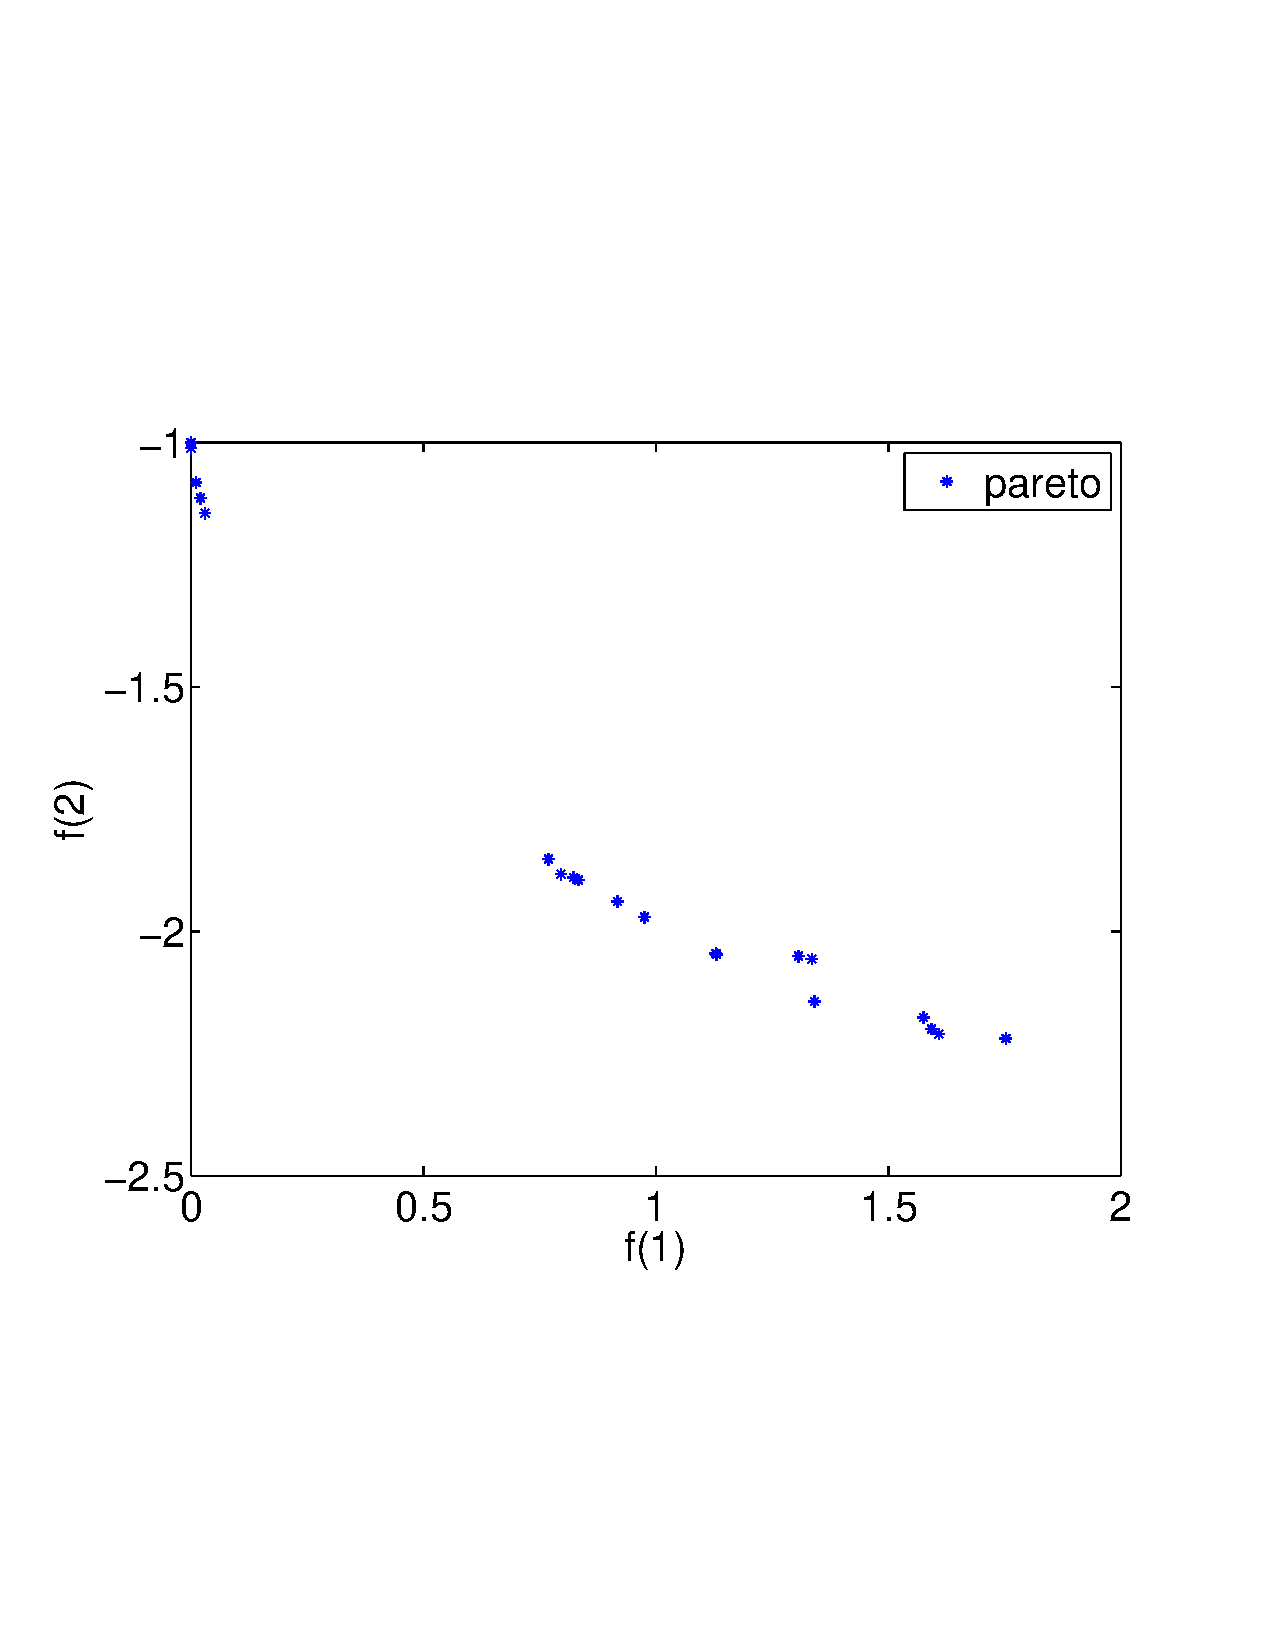
\includegraphics[width=100mm]{pareto_nsga-ii.pdf}
\caption{NSGA-2 Curva Pareto para o quadrado do raio de duas fun��es de c�rculos conc�ntricos: $f_1$, em torno de (0,0) e $f_2$ em torno de (1,0).}
\label{perfil}
\end{figure}	

\section{Otimiza��es por for�a bruta: gerando base de \textbf{f}(\textbf{x}) para testes}
O principal objetivo deste trabalho, foi gerar uma base de dados com valores de dom�nio e imagem das fun��es objetivos de testes, encontradas na literatura. Foram geradas as otimiza��es demonstradas nas figuras abaixo sem nenhuma t�cnica evolucion�ria. Apenas uma nuvem de pontos aleat�rios foram lan�adas no espa�o, e os valores de $f_1$ e $f_2$ foram plotados. Depois, apenas os pontos n�o dominados foram plotados na cor vermelha.
A base de dados, com dez pontos de cada fun��o teste, encontra-se no arquivo ``bd.zip''.\textbf{ Lembrem-se: as primeiras colunas dos arquivos txt  correspondem aos valores de \textbf{x} e as duas �ltimas colunas s�o os valores correspondentes de }$f_1$ e $f_2$.

\newpage
\subsection{SCH: }
\begin{figure}[h!]
\centering
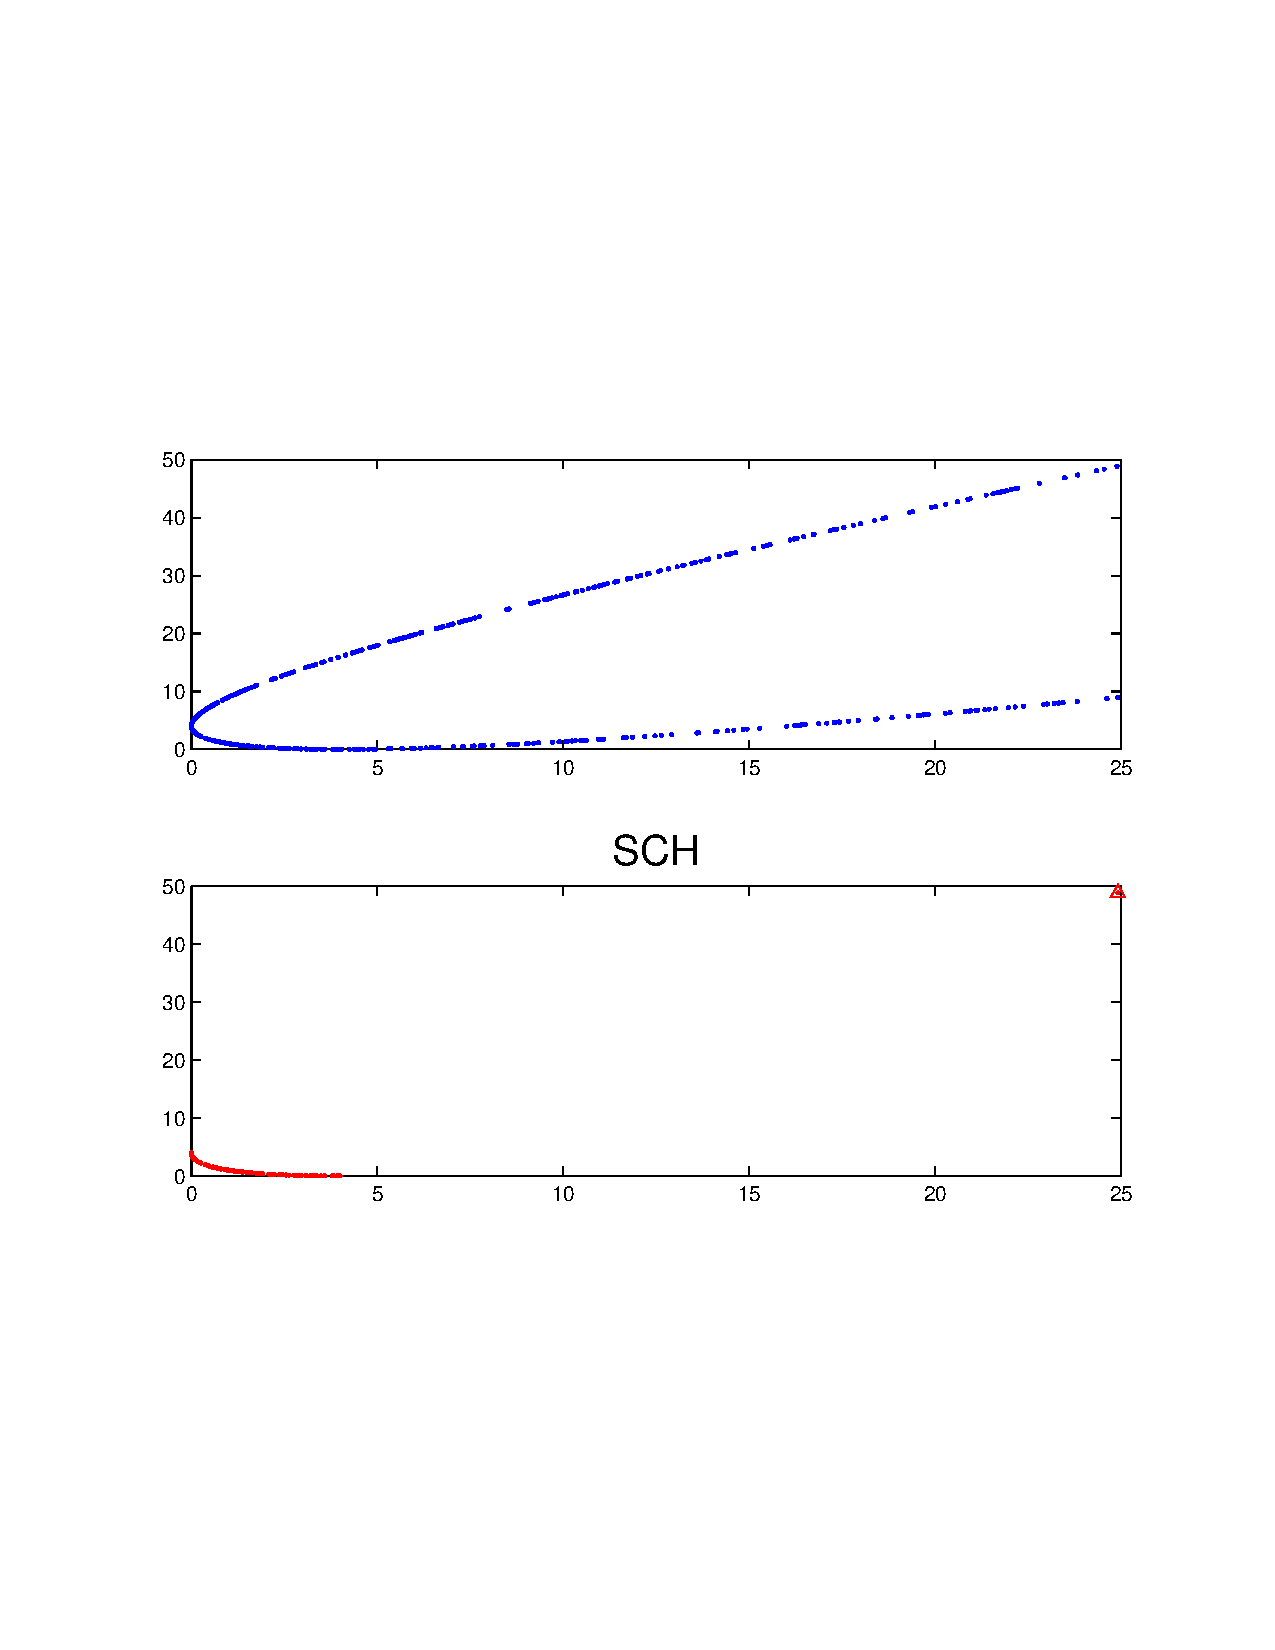
\includegraphics[width=180mm]{SCH.pdf}
\label{perfil}
\end{figure}

\newpage
\subsection{FON: }
\begin{figure}[h!]
\centering
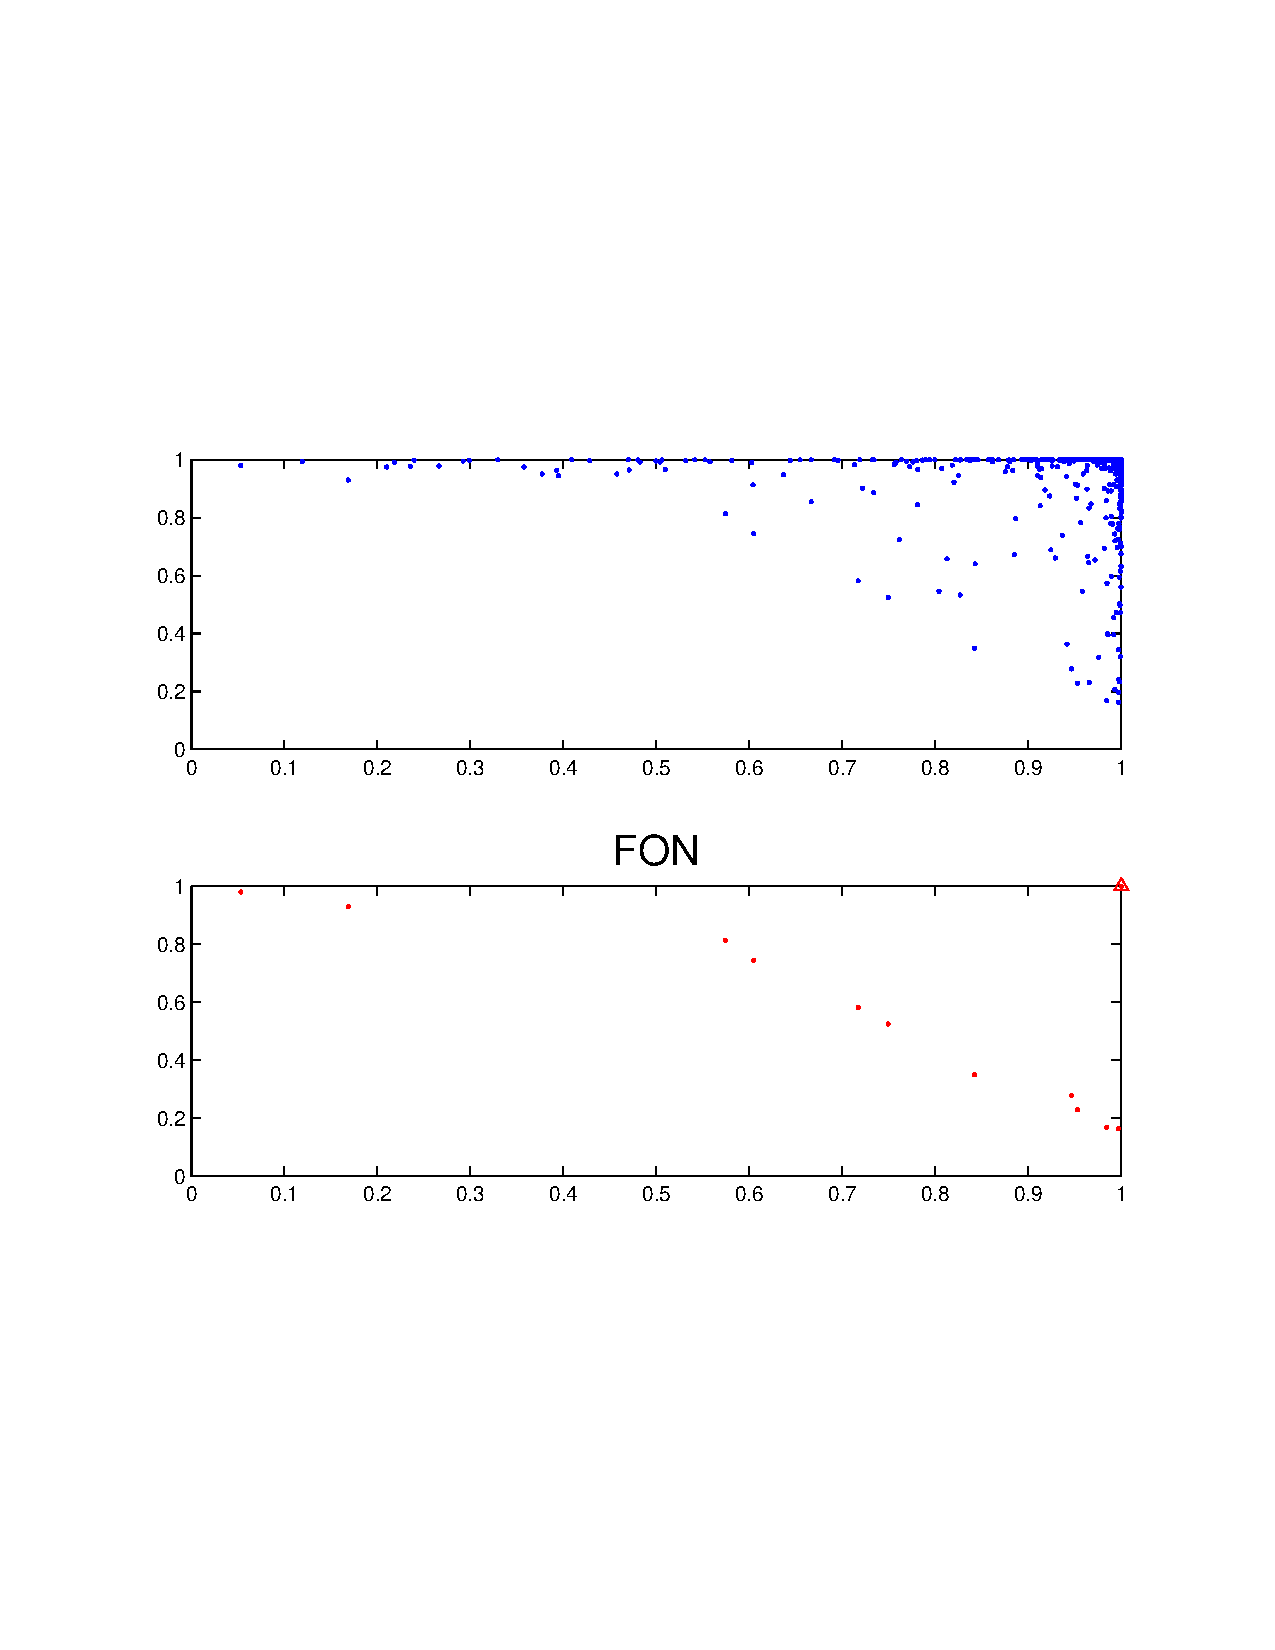
\includegraphics[width=180mm]{FON.pdf}
\label{perfil}
\end{figure}

\newpage
\subsection{POL: }
\begin{figure}[h!]
\centering
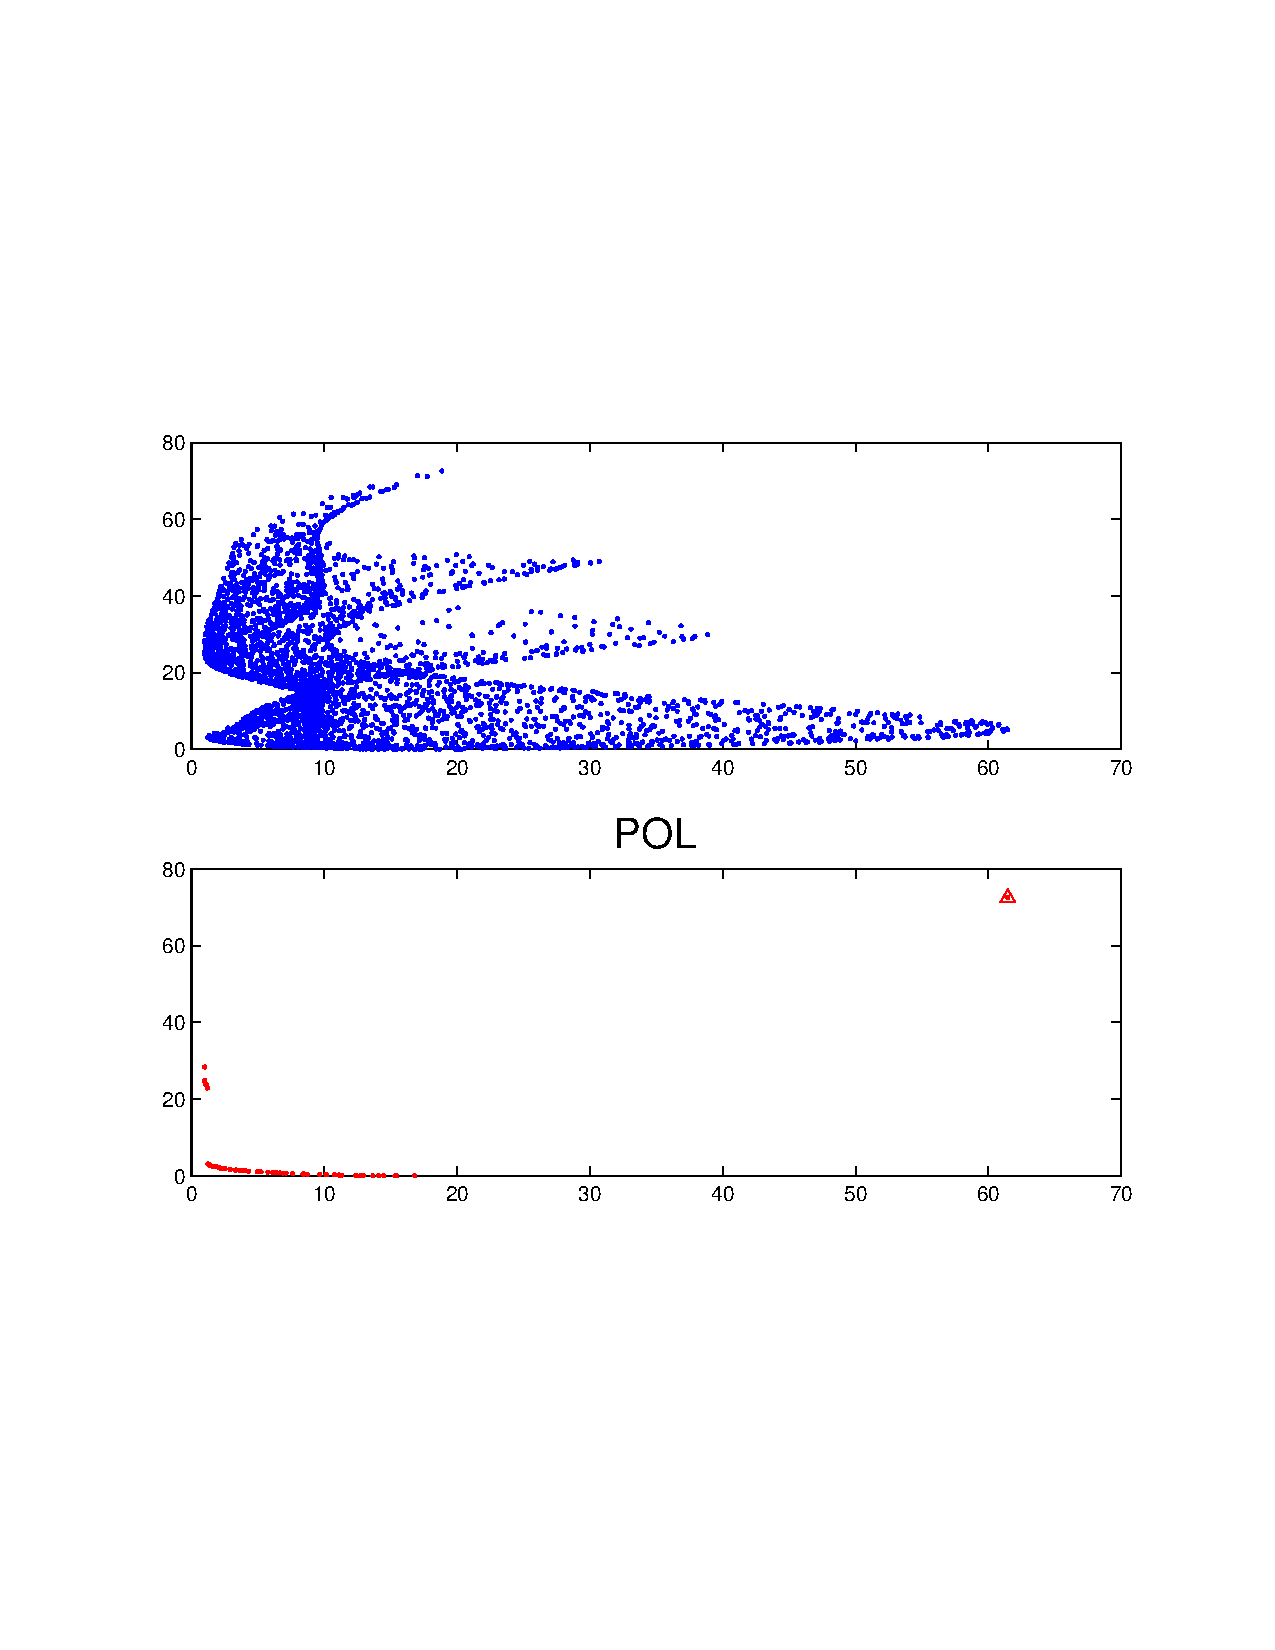
\includegraphics[width=180mm]{POL.pdf}
\label{perfil}
\end{figure}

\newpage
\subsection{KUR: }
\begin{figure}[h!]
\centering
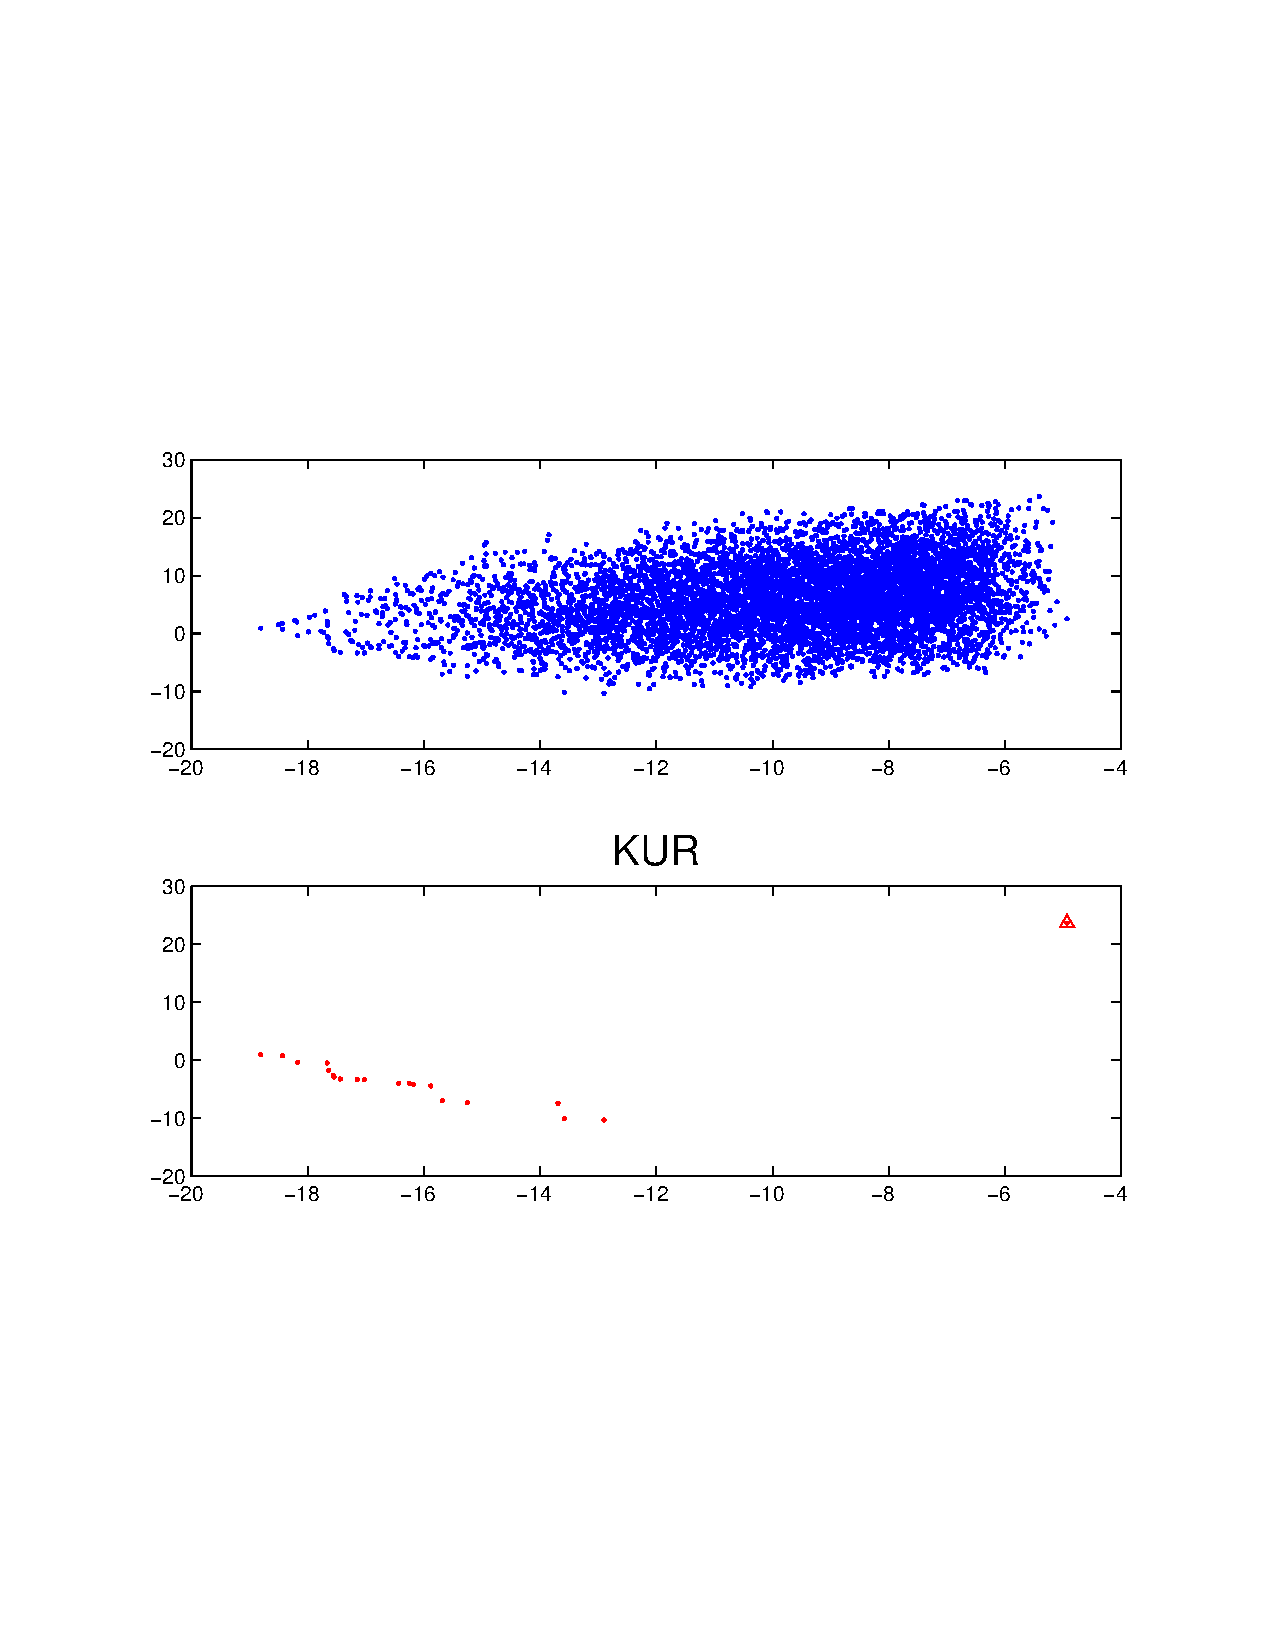
\includegraphics[width=180mm]{KUR.pdf}
\label{perfil}
\end{figure}

\newpage
\subsection{ZDT1: }
\begin{figure}[h!]
\centering
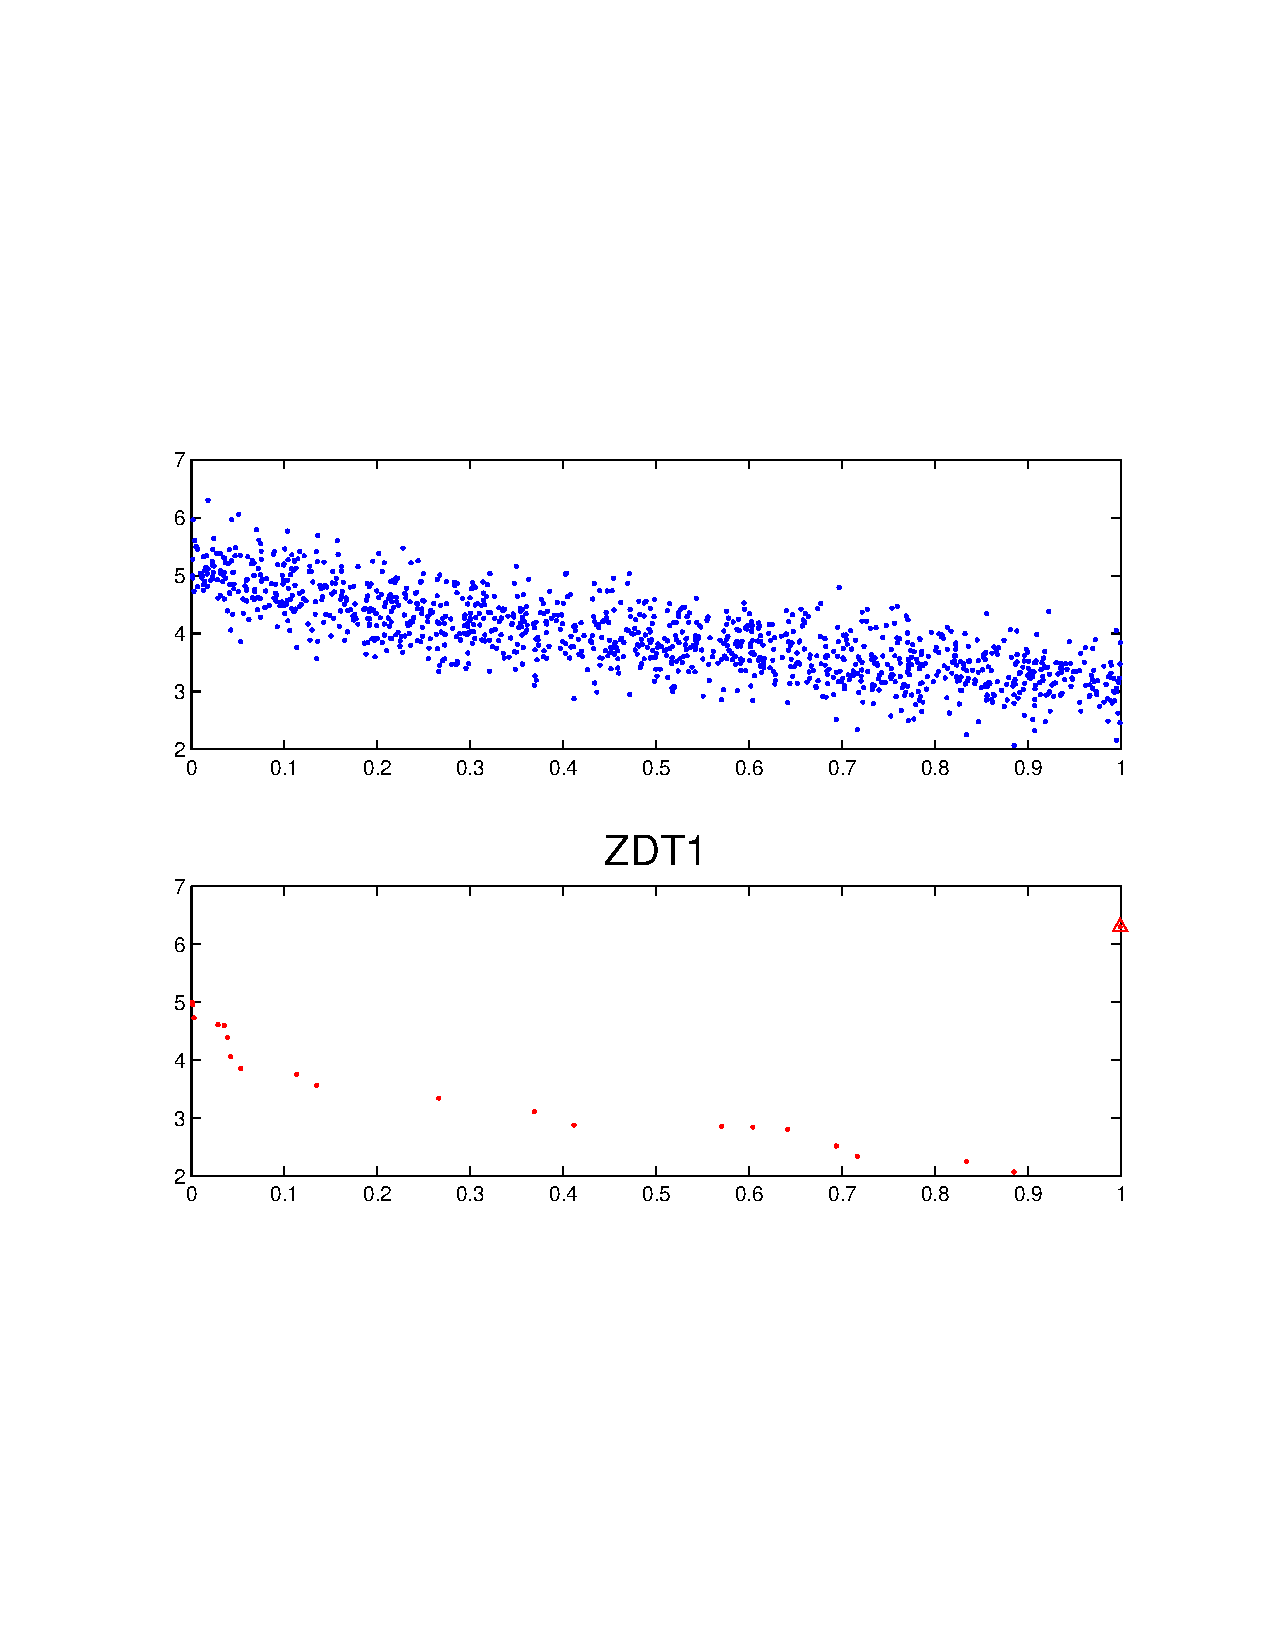
\includegraphics[width=180mm]{ZDT1.pdf}
\label{perfil}
\end{figure}

\newpage
\subsection{ZDT2: }
\begin{figure}[h!]
\centering
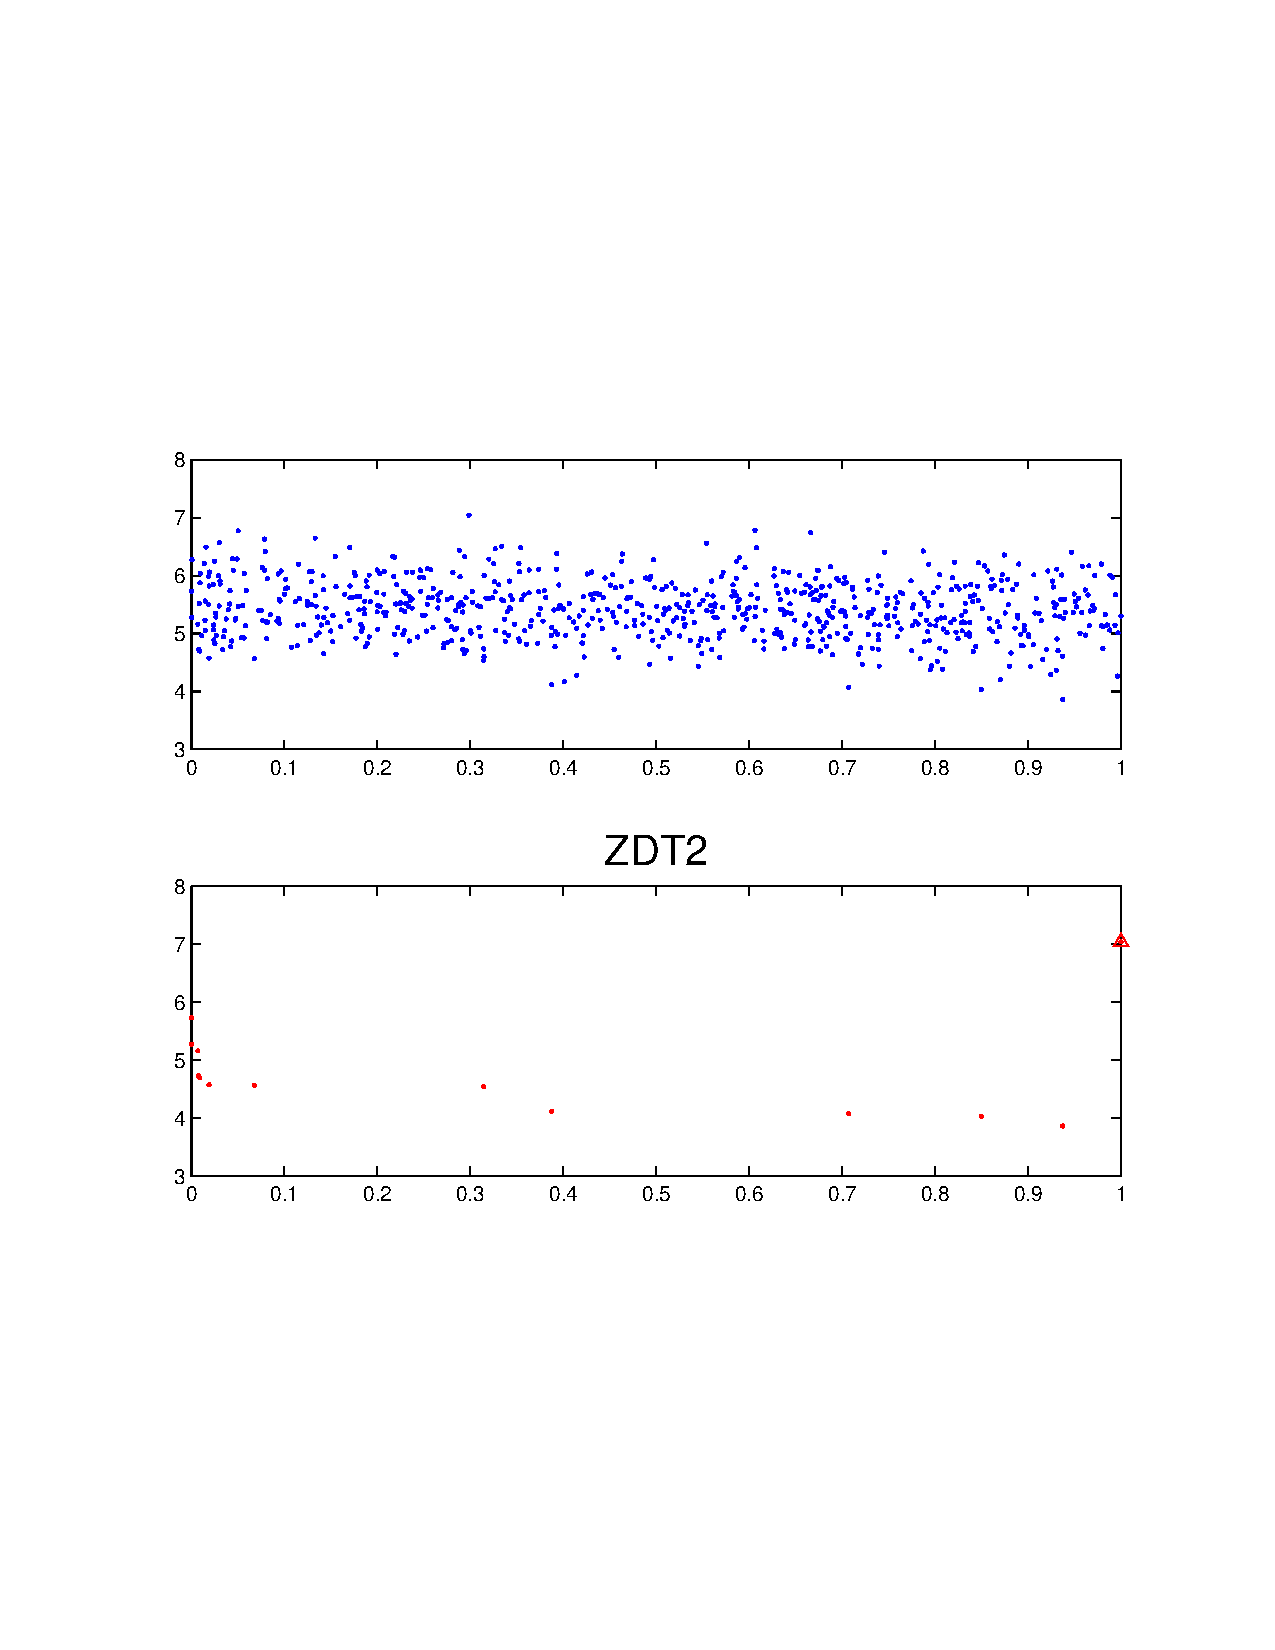
\includegraphics[width=180mm]{ZDT2.pdf}
\label{perfil}
\end{figure}

\newpage
\subsection{ZDT3: }
\begin{figure}[h!]
\centering
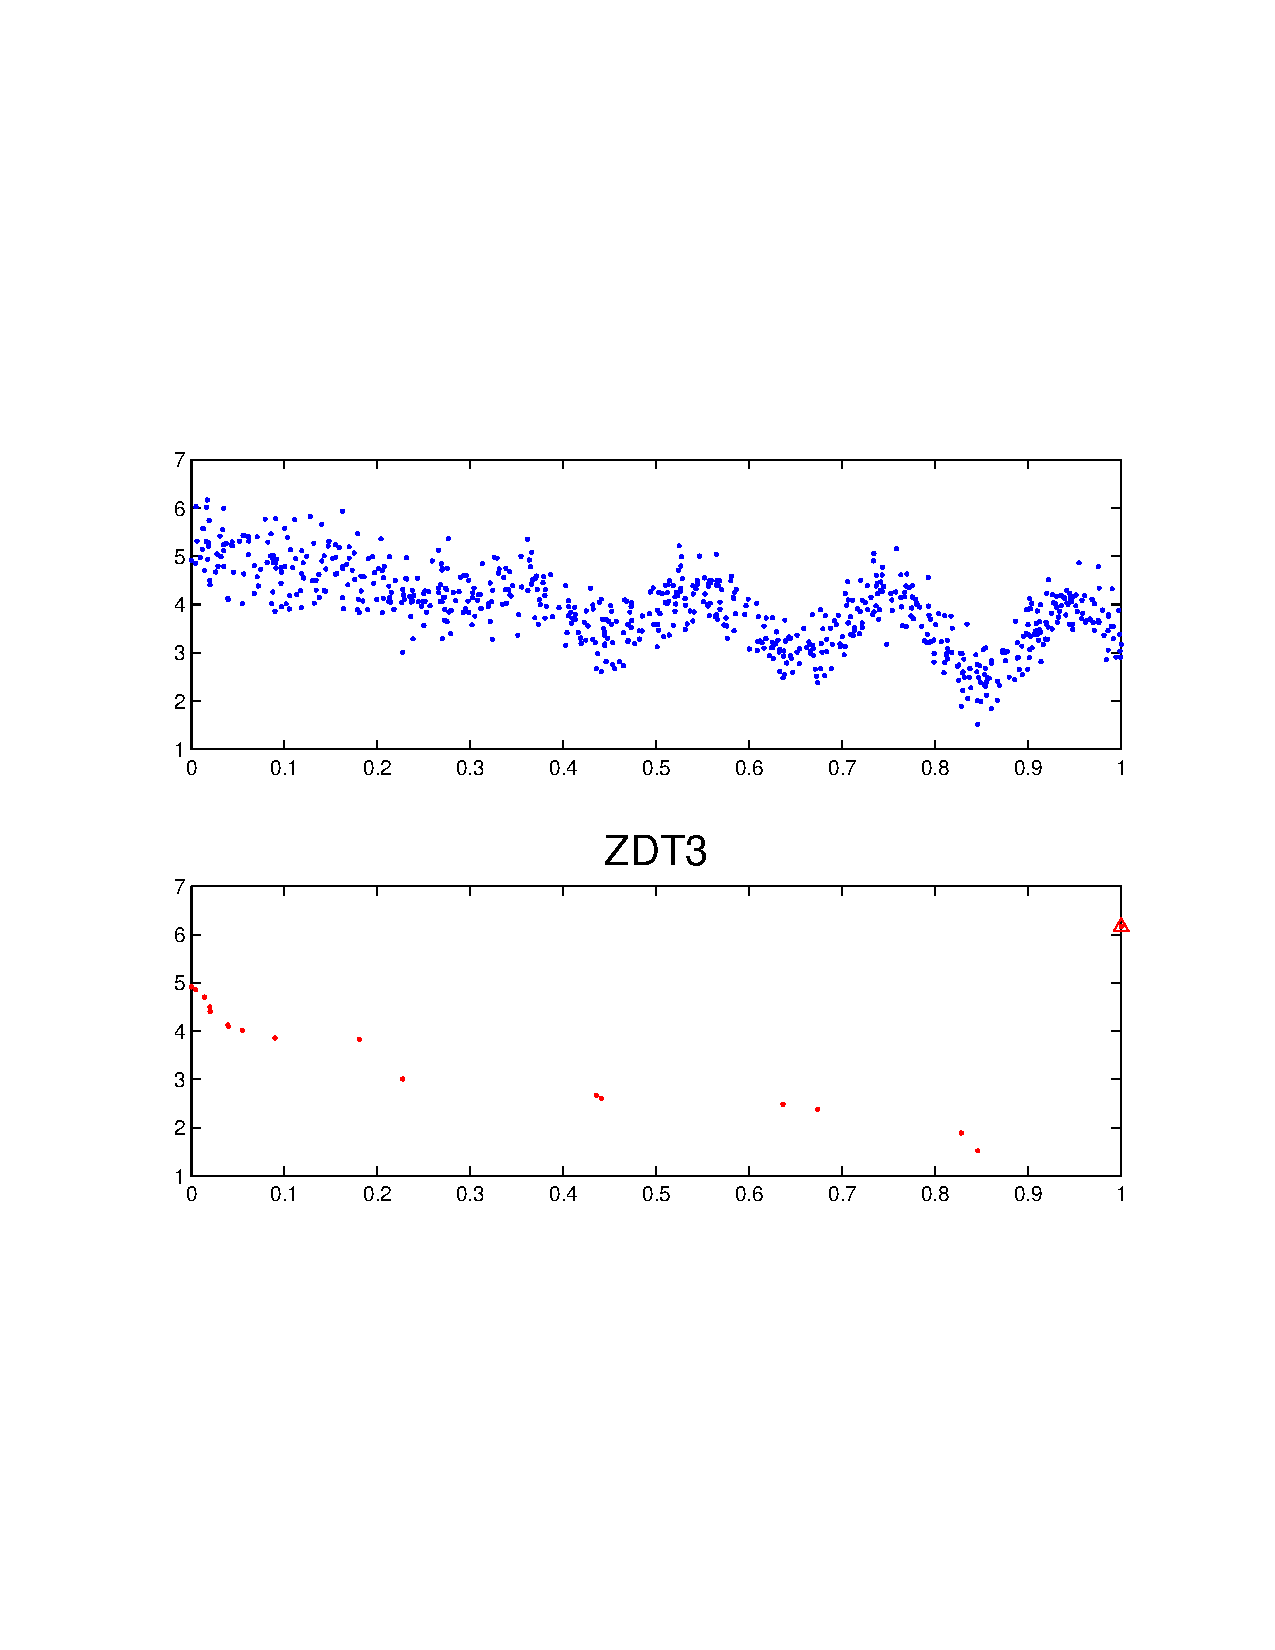
\includegraphics[width=180mm]{ZDT3.pdf}
\label{perfil}
\end{figure}

\newpage
\subsection{ZDT4: }
\begin{figure}[h!]
\centering
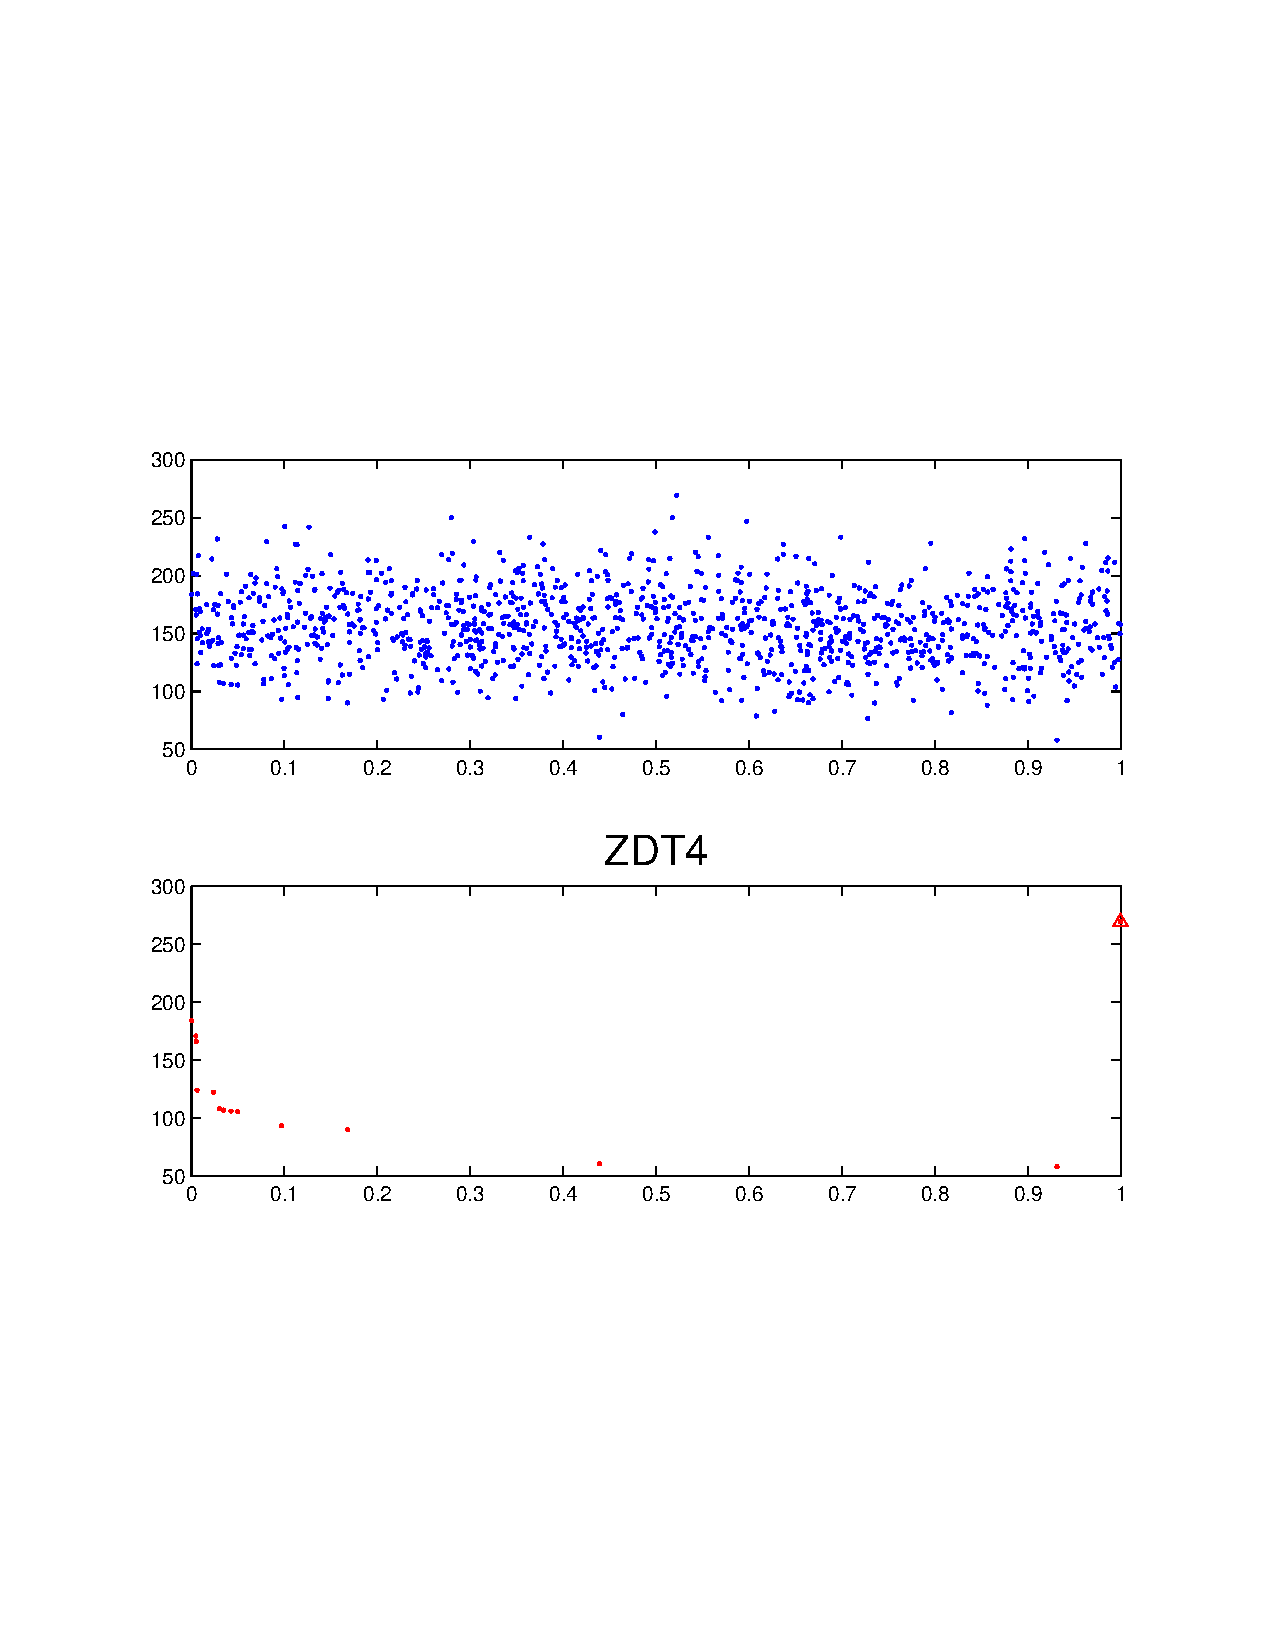
\includegraphics[width=180mm]{ZDT4.pdf}
\label{perfil}
\end{figure}

\newpage
\subsection{ZDT6: }
\begin{figure}[h!]
\centering
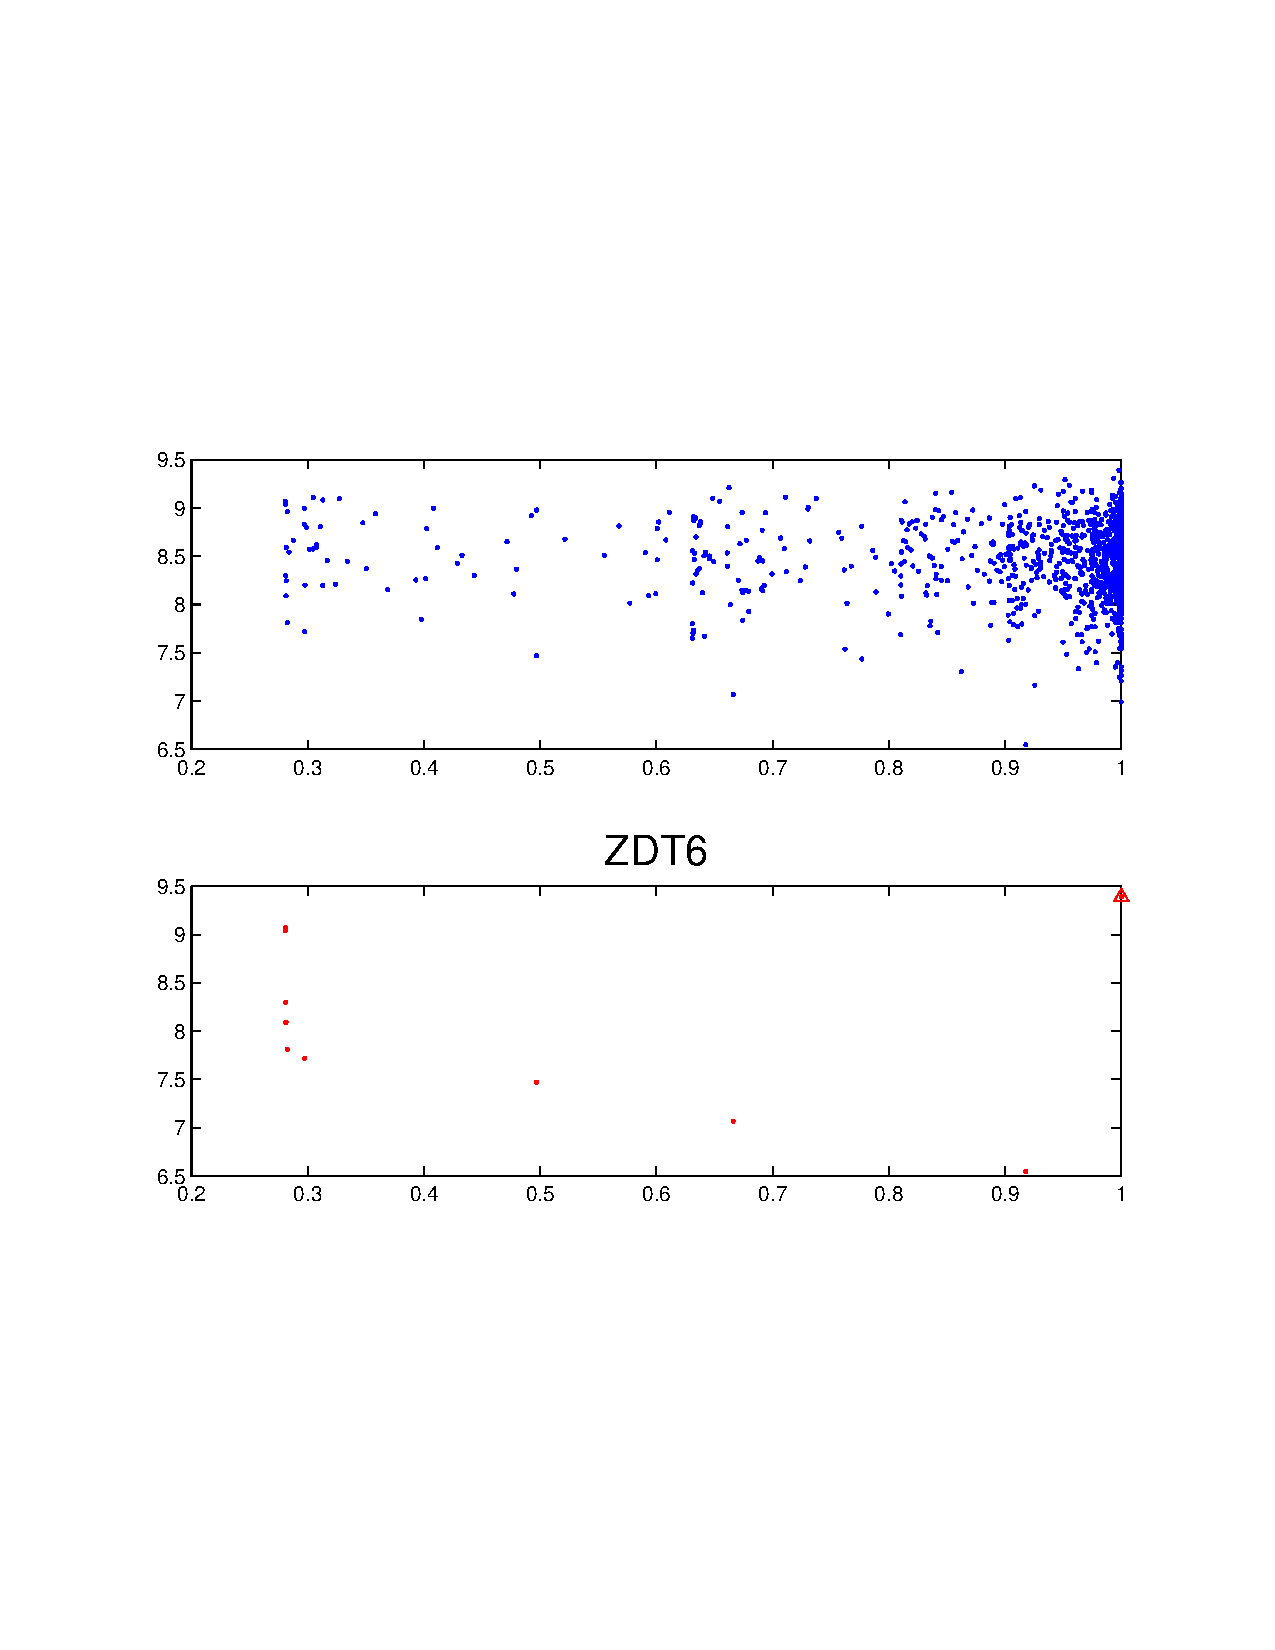
\includegraphics[width=180mm]{ZDT6.pdf}
\label{perfil}
\end{figure}

\end{document}




